\documentclass[a4paper,12pt]{report} 
\usepackage[french]{babel} 
\usepackage{xcolor,graphicx}
\usepackage[top=0.6in,bottom=0.6in,right=1in,left=1in]{geometry}
\usepackage[top=0.6in,bottom=0.6in,right=1in,left=1in]{geometry}
\usepackage[T1]{fontenc}
\usepackage[utf8]{inputenc}
\usepackage[utf8]{inputenc}
\usepackage{xcolor,graphicx}
\usepackage{fancyhdr}
\usepackage{listings}
\usepackage{array}
\usepackage{adjustbox}
\usepackage[colorlinks, allcolors=black]{hyperref}
\usepackage{lipsum}
\usepackage{amsmath}
\usepackage{caption}
\usepackage{enumitem}
\setlength{\headheight}{14.61858pt}
\definecolor{blue}{RGB}{31,56,100}
\hypersetup{
    pdftitle={Titre de la mémoire},    % Titre 
    pdfauthor={Nom Prénom},    % Auteur
    pdfsubject={Domaine},   % Sujet 
    pdfkeywords={keyword1, keyword2},   % liste Mot clés
}

%%%%%%%%%%%%%%%%%%%%%%%%%%%%%%%%%%%%%%%%%%%%%%%%%%%%%%%%%%%%%%%%%%%%%%%%%%%%%
%%%%%%%%%%%%%%%%%%%%%%%%%%%%%%%%%%%%%%%%%%%%%%%%%%%%%%%%%%%%%%%%%%%%%%%%%%%%
%% Modifier Selon vos informations visibles (Choisir un titre bref et précis)
\newcommand{\mytitle}{Système de recommandation basé sur l'IA générative}
\newcommand{\myname}{M. Zarouala Abdellah}
\newcommand{\mylogo}{
\includegraphics[height=1.8cm]{./images/Ste_logo.jpg}} 

%%%%%%%%%%%%%%%%%%%%%%%%%%%%%%%%%%%%%%%%%%%%%%%%%%%%%%%%%%%
% Numérotation des sections de début
\fancypagestyle{firstpages}{
    \fancyhf{}  
    \renewcommand{\headrulewidth}{0pt}  
    \fancyfoot[C]{\thepage}  
    \pagenumbering{arabic}  
}

% Numérotation des chapitres
 

% Style pour le code listings
\definecolor{codegreen}{rgb}{0,0.6,0}
\definecolor{codegray}{rgb}{0.5,0.5,0.5}
\definecolor{codepurple}{rgb}{0.58,0,0.82}
\definecolor{backcolour}{rgb}{0.95,0.95,0.92}

\lstdefinestyle{mystyle}{
    backgroundcolor=\color{backcolour},   
    commentstyle=\color{codegreen},
    keywordstyle=\color{magenta},
    numberstyle=\tiny\color{codegray},
    stringstyle=\color{codepurple},
    basicstyle=\ttfamily\footnotesize,
    breakatwhitespace=false,         
    breaklines=true,                 
    captionpos=b,                    
    keepspaces=true,                 
    numbers=left,                    
    numbersep=5pt,                  
    showspaces=false,                
    showstringspaces=false,
    showtabs=false,                  
    tabsize=2
}
\lstset{style=mystyle}


%%%%% Profendeur des sections
\setcounter{tocdepth}{3}
\setcounter{secnumdepth}{3}

\begin{document}
%%%%%%%%%%%%%%%%%%%%%%%%%%%%%%%%%%%%%%%%%%%%%%%%%%%%%%%%%%%%%%%%%%%%%%%%%%%%%%
%%%%%%%%%%%%%%%%%%%%%%%%%%%%%%%%%%%%%%%%%%%%%%%%%%%%%%%%%%%%%%%%%%%%%%%%%%%%%%
% Page de Garde
%%%%%%%%%%%%%%%%%%%%%%%%%%%%%%%%%%%%%%%%%%%%%%%%%%%%%%%%%%%%%%%%%%%%%%%%%%%%%
%%%%%%%%%%%%%%%%%%%%%%%%%%%%%%%%%%%%%%%%%%%%%%%%%%%%%%%%%%%%%%%%%%%%%%%%%%%%%
%%%% Entéte Logo de l'université Mohammed V - Faculté des sciences Rabat
\begin{titlepage}
    \begin{center}
        \begin{minipage}{3cm}
            \begin{center}
            
\includegraphics[height=1.8cm]{./images/Logo_FSR.jpg}
            \end{center}
        \end{minipage} \hfill
        \begin{minipage}{9cm}
            \begin{center}
            \textbf{UNIVERSITÉ MOHAMMED V }\\[0.1cm]
            \textbf{FACULTÉ DES SCIENCES RABAT}\\[0.1cm]
            \textbf{DÉPARTEMENT D'INFORMATIQUE}
            \end{center}
        \end{minipage}\hfill
        \begin{minipage}{3cm}
            \begin{center}
            
\includegraphics[height=1.3cm]{./images/Logo_MSID_invisible.png}
        \end{center}
        \end{minipage}
    %%%%%%%%%%%%%%%%%%%%%%%%%%%%%%%%%%%%%%%%%%%%%%%%%%%%%%%%%%%%%%%%%%%%%%%%%%%%%%%%%%%
    %%%%%%%%%%%%%%%%%%%%%%%%%%%%%%%%%%%%%%%%%%%%%%%%%%%%%%%%%%%%%%%%%%%%%%%%%%%%%%%%%%%
    \textsc{\Large }\\[1.5cm]
    {\large \bfseries Mémoire du Projet de Fin d'\uppercase{é}tudes}\\[0.5cm]
    {\large En vue de l'obtention du diplôme}\\[1cm]
    {\huge \bfseries \uppercase{Master Science et Ingénierie de Données} \\[0.5cm] }
    %%%%%%%%%%%%%%%%%%%%%%%%%%%%%%%%%%%%%%%%%%%%%%%%%%%%%%%%%%%%%%%%%%%%%%%%%%%%%%%%%%%
    %%%%%%%%%%%%%%%%%%%%%%%%%%%%%%%%%%%%%%%%%%%%%%%%%%%%%%%%%%%%%%%%%%%%%%%%%%%%%%%%%%%
    %% Ajouter votre Nom et Prénom
    \begin{center} 
    \large
    \emph{Présenté(e) par } \\ [0.2cm]
        \bfseries \textbf{\myname}\\
      \end{center} 
    %%%%%%%%%%%%%%%%%%%%%%%%%%%%%%%%%%%%%%%%%%%%%%%%%%%%%%%%%%%%%%%%%%%%%%%%%%%%%%%
    %%%%%%%%%%%%%%%%%%%%%%%%%%%%%%%%%%%%%%%%%%%%%%%%%%%%%%%%%%%%%%%%%%%%%%%%%%%%%%
    {\large \bfseries   Sous le thème :}\\[0.5cm]
    
    %%%%%%%%%%%%%%%%%%%%%%%%%%%%%%%%%%%%%%%%%%%%%%%%%%%%%%%%%%%%%%%%%%%%%%%%%%%%%%%%%%%%%%%%%%%%%%%%%%%%%%%%%%%%%%%%%%%%%%%%%%%%%%%%%%%%%%%%%%%%%%%%%%%%%%%%%%
    %% Ajouter le titre de votre sujet (Ne pas dépassé trois lignes)
    \rule{\linewidth}{0.3mm} \\[0.4cm]
    { \huge \bfseries\color{blue} \mytitle \\[0.4cm] }
    \rule{\linewidth}{0.3mm} \\[1cm]
    
    %%%%%%%%%%%%%%%%%%%%%%%%%%%%%%%%%%%%%%%%%%%%%%%%%%%%%%%%%%%%%%%%%%%%%%%%%%%%%%
    %%%%%%%%%%%%%%%%%%%%%%%%%%%%%%%%%%%%%%%%%%%%%%%%%%%%%%%%%%%%%%%%%%%%%%%%%%%%%%%
    %% Vous pouvez supprimer ces balises si vous n'en avez pas besoin
    %% Le logo de la société doit être conforme aux dimensions du fichier Ste_logo.jpg
    \begin{center}
    \begin{minipage}{\linewidth}
    \begin{flushright}
   
    \end{flushright}   
    \end{minipage}\\[2cm]
    \end{center} 
    %%%%%%%%%%%%%%%%%%%%%%%%%%%%%%%%%%%%%%%%%%%%%%%%%%%%%%%%%%%%%%%%%%%%%%%%%%%%%%%
    %%%%%%%%%%%%%%%%%%%%%%%%%%%%%%%%%%%%%%%%%%%%%%%%%%%%%%%%%%%%%%%%%%%%%%%%%%%%%%
    %% Modifier la date du soutenance
    {\large \textit{Soutenu le 12 Juillet 2025, devant le jury composé de : }}\\[0.5cm]
    \color{black}
    %%%%%%%%%%%%%%%%%%%%%%%%%%%%%%%%%%%%%%%%%%%%%%%%%%%%%%%%%%%%%%%%%%%%%%%%%%%%%%%
    %%%%%%%%%%%%%%%%%%%%%%%%%%%%%%%%%%%%%%%%%%%%%%%%%%%%%%%%%%%%%%%%%%%%%%%%%%%%%%
    %% Modifier les noms de la comité du soutenance
   
\begin{tabular}{>{\arraybackslash}m{6.5cm} >{\arraybackslash}m{5cm} >{\arraybackslash}m{5.5cm}}
        \large \textbf{Pr.}~\textsc{Soumia}   ZITI   & PES, FSR - UM5R & \large \textbf{Présidente} \\[0.1cm]
        \large \textbf{Pr.}~\textsc{Nassim}  KHARMOUM & MCH, FSR - UM5R      & \large \textbf{Encadrant interne} \\[0.1cm] 
        \large \textbf{Dr.}~\textsc{Wafae} ABBAOUI      & MC EMSI & \large \textbf{Examinatrice} \\[0.1cm]     
        \large \textbf{Dr.}~\textsc{Mohammed} AMRAOUI      & Docteur, FSR - UM5R & \large \textbf{Examinateur} \\[0.1cm]   
    \end{tabular}
    
    \vfill
    %%%%%%%%%%%%%%%%%%%%%%%%%%%%%%%%%%%%%%%%%%%%%%%%%%%%%%%%%%%%%%%%%%%%%%%%%%%%%%
    %%%%%%%%%%%%%%%%%%%%%%%%%%%%%%%%%%%%%%%%%%%%%%%%%%%%%%%%%%%%%%%%%%%%%%%%%%%%%%
    %% Pied de la page de Garde
    {\textbf{\large {Année universitaire} 2024-2025}}
    \end{center}
    \end{titlepage}
\pagestyle{firstpages}
% Page de Remerciements
%%%%%%%%%%%%%%%%%%%%%%%%%%%%%%%%%%%%%%%%%%%%%%%%%%%%%%%%%%%%%%%%%%%%%%%%%%
%%%%%%%%%%%%%%%%%%%%%%%%%%%%%%%%%%%%%%%%%%%%%%%%%%%%%%%%%%%%%%%%%%%%%%%%%%%
% Page de Remerciements
\newgeometry{top=0.6in,bottom=0.6in,right=1in,left=1in}


\chapter*{Dédicace}
% Your dedication text goes here...
\addcontentsline{toc}{chapter}{Dédicace}
\begin{flushright}
\rule{\linewidth}{0.1mm} \\[0.4cm]
\textit{Je tiens à remercier toutes les personnes qui m'ont aidé à réaliser ce travail.\\[0.5cm]
\lipsum[3]}
\rule{\linewidth}{0.1mm} \\[0.4cm]
\end{flushright}
\vspace*{\fill}

\restoregeometry



% Page de Résumé

%%%%%%%%%%%%%%%%%%%%%%%%%%%%%%%%%%%%%%%%%%%%%%%%%%%%%%%%%%%%%%%%%%%%%%%%%%%%
%%%%%%%%%%%%%%%%%%%%%%%%%%%%%%%%%%%%%%%%%%%%%%%%%%%%%%%%%%%%%%%%%%%%%%%%%%%%
% Page de Résumé en francais
 

\chapter*{Résumé}
\addcontentsline{toc}{chapter}{Résumé}

\paragraph{}\begin{spacing}{2}

La plupart des plateformes d’enseignement en ligne encouragent leurs utilisateurs à explorer différentes thématiques avant de s’engager dans une spécialisation, et à développer une culture académique large en suivant des parcours diversifiés. Chaque période, les apprenants doivent choisir, parmi des milliers de cours disponibles dans de nombreux domaines, une sélection restreinte de formations à suivre. L’environnement en ligne est également très dynamique, et une communication insuffisante ainsi que des fonctions de recherche peu performantes peuvent limiter la capacité des apprenants à découvrir de nouveaux cours adaptés à leurs intérêts.

Pour aider à la fois les apprenants et les conseillers pédagogiques dans ce contexte, nous explorons un système novateur de recommandation de cours en ligne basé sur un grand modèle de langage (LLM) utilisant une méthode de \textit{Retrieval Augmented Generation} (RAG) appliquée au corpus des descriptions de cours. Le système génère d’abord une description de cours « idéale » à partir de la requête ou du profil de l’utilisateur. Cette description est convertie en un vecteur de recherche via des embeddings, qui est ensuite utilisé pour retrouver des cours réels au contenu similaire en comparant les similarités d’embeddings.

Nous décrivons la méthode et évaluons la qualité ainsi que la pertinence de certains exemples de requêtes. Les étapes pour déployer un système pilote sur une plateforme d’apprentissage en ligne sont également discutées.

\medskip

\textbf{Mots-clés :} systèmes de recommandation, grands modèles de langage, génération augmentée par récupération, technologie éducative, recommandation de cours en ligne
\end{spacing}

\newpage
%%%%%%%%%%%%%%%%%%%%%%%%%%%%%%%%%%%%%%%%%%%%%%%%%%%%%%%%%%%%%%%%%%%%%%%%%%%%
%%%%%%%%%%%%%%%%%%%%%%%%%%%%%%%%%%%%%%%%%%%%%%%%%%%%%%%%%%%%%%%%%%%%%%%%%%%%
% Page de Abstract en anglais

%%%%%%%%%%%%%%%%%%%%%%%%%%%%%%%%%%%%%%%%%%%%%%%%%%%%%%%%%%%%%%%%%%%%%%%%%%%%%
%%%%%%%%%%%%%%%%%%%%%%%%%%%%%%%%%%%%%%%%%%%%%%%%%%%%%%%%%%%%%%%%%%%%%%%%%%%%%
% Page de Abstract

\chapter*{Abstract}
\addcontentsline{toc}{chapter}{Abstract}
\paragraph{}
\textit{The abstract of your work in English.} \\[0.5cm]
\lipsum[1-2] \\
\textbf{Keywords :} Keyword 1, Keyword 2, Keyword 3, Keyword 4, Keyword 5

\newpage
%%%%%%%%%%%%%%%%%%%%%%%%%%%%%%%%%%%%%%%%%%%%%%%%%%%%%%%%%%%%%%%%%%%%%%%%%%%%%%%%%%%%%%%%%%%%%%%%%%%%%%%%%%%%%%%%%%%%%%%%%%%%%%%%%%%%%%%%%%%%%%%%%%%%%%%%%%
% Table des matières
\phantomsection
\tableofcontents
\addcontentsline{toc}{chapter}{Table des matières}
\newpage

% Liste des figures
\phantomsection
\listoffigures
\addcontentsline{toc}{chapter}{Liste des figures}
\newpage

% Liste des tableaux
\phantomsection
\addcontentsline{toc}{chapter}{Liste des tableaux}
\listoftables
\newpage

%%%%%%%%%%%%%%%%%%%%%%%%%%%%%%%%%%%%%%%%%%%%%%%%%%%%%%%%%%%%%%%%%%%%%%%%%%%%
%%%%%%%%%%%%%%%%%%%%%%%%%%%%%%%%%%%%%%%%%%%%%%%%%%%%%%%%%%%%%%%%%%%%%%%%%%%%
  
% Introduction
%%%%%%%%%%%%%%%%%%%%%%%%%%%%%%%%%%%%%%%%%%%%%%%%%%%%%%%%%%%%%%%%%%%%%%%%%%%%%
%%%%%%%%%%%%%%%%%%%%%%%%%%%%%%%%%%%%%%%%%%%%%%%%%%%%%%%%%%%%%%%%%%%%%%%%%%%%%
% Introduction
\chapter*{Introduction Générale}
\addcontentsline{toc}{chapter}{Introduction Générale}
\paragraph{}
\lipsum[1-3]
\newpage

%%%%%%%%%%%%%%%%%%%%%%%%%%%%%%%%%%%%%%%%%%%%%%%%%%%%%%%%%%%%%%%%%%%%%%%%%%%
% Chapitre 1
\chapter{Chapitre 1 : Intelligence artificielle générative}
%%%% Intro du Chapitre
\phantomsection
\section*{Introduction}
\addcontentsline{toc}{section}{Introduction}
\paragraph{}
En quoi consiste l’IA générative ? L'intelligence artificielle générative est
une catégorie d'IA qui se concentre sur la création autonome de contenu, tels que
des textes, des images, des vidéos, des sons et d'autres types de données, par des
systèmes informatiques.

Ces systèmes utilisent des modèles avancés d'apprentissage automatique pour générer
du contenu qui peut ressembler à ce qui est créé par des êtres humains.
\section{Quelles techniques sont utilisées dans l’IA générative ?}
\paragraph{}
Les deux types d'IA générative les plus utilisées sont :

\begin{itemize}
	\item \textbf{Les GAN (neurones génératifs antagonistes)} : une architecture
		de réseau de neurones artificiels composée de deux parties, le générateur et
		le discriminant. Le générateur crée de nouvelles données, tandis que le discriminant
		essaie de distinguer les données générées de données réelles. Les GAN s'améliorent
		continuellement à mesure que le générateur tente de tromper le discriminant,
		créant ainsi des données de plus en plus réalistes. Les GAN sont couramment
		utilisés pour générer des images, des vidéos et des textes.

	\item \textbf{Les GPT (Generative Pre-trained Transformer)} : des modèles d'apprentissage
		automatique qui ont été formés sur de grandes quantités de données
		textuelles. Ces modèles peuvent générer du texte cohérent et contextuellement
		pertinent en fonction des données d'entrée. Ils sont utilisés pour des
		applications telles que la génération automatique de textes, la traduction automatique
		et la rédaction assistée par ordinateur.
\end{itemize}
\section{A quoi sert l'IA générative ?}
\paragraph{}
Les applications de l'IA générative sont nombreuses et très diverses. Elle peut
servir pour :

\begin{itemize}[label=--]
	\item \textbf{Alimenter la création artistique} : en générant de l'art visuel,
		de la musique, de la littérature et d'autres formes d'expression artistique
		;

	\item \textbf{Améliorer la création de contenu} : en aidant les rédacteurs à
		générer du contenu rédactionnel, tels que des articles, des rapports ou même
		des scripts pour la création de vidéos ;

	\item \textbf{Créer des mondes virtuels} : des personnages et des scénarios
		dans des jeux vidéo et des simulations ;

	\item \textbf{Personnaliser l'expérience utilisateur} : en tenant compte des
		préférences individuelles de chaque utilisateur ;

	\item \textbf{Générer des données de test} : en informatique ou en science ;

	\item \textbf{Coder des programmes simples} : grâce notamment au \textit{no-code},
		et remplacer le \textit{low-code}.
\end{itemize}
\section{Quels sont les inconvénients de l’IA générative ?}
\paragraph{}
Les concepteurs, les développeurs et les utilisateurs de ces systèmes doivent également
être conscients des implications éthiques et sociales et veiller à une utilisation
responsable de cette technologie. Voici quelques-uns des principaux
inconvénients à avoir en tête :
\begin{itemize}[label=--]
	\item \textbf{Qualité variable du contenu} : Les résultats générés par des
		modèles d'IA générative peuvent varier en termes de qualité et de pertinence.
		Il est possible d'obtenir du contenu de qualité médiocre, trompeur ou
		inutile. L'IA générative peut être utilisée de manière malveillante pour créer
		de la désinformation, des \textit{deepfakes} et d'autres formes de manipulation
		de contenu. La source du contenu généré peut être remise en question, affectant
		la confiance du public dans les informations en ligne.

	\item \textbf{Problèmes de responsabilité} : Déterminer la responsabilité en
		cas de contenu inapproprié ou problématique généré par une IA peut être
		complexe, notamment lorsqu'il s'agit de modèles pré-entraînés sur de vastes ensembles
		de données.

	\item \textbf{Surcharge d'informations} : L'IA générative peut générer un
		volume massif de contenu, ce qui complique la recherche d'informations pertinentes.

	\item \textbf{Biais et discrimination} : Les modèles peuvent reproduire les
		biais présents dans les données d'entraînement, entraînant la création de contenu
		discriminatoire, offensant ou partial.

	\item \textbf{Menace pour l'emploi} : Dans certains secteurs, l'automatisation
		de la création de contenu peut mener à la suppression d'emplois (rédaction, conception
		graphique, etc.).

	\item \textbf{Problèmes de sécurité} : Les cybercriminels peuvent exploiter l'IA
		générative pour créer des contrefaçons, des faux documents ou des attaques de
		\textit{phishing} plus sophistiquées.

	\item \textbf{Défis éthiques} : Des questions importantes se posent en matière
		de propriété intellectuelle, de création automatisée sans consentement, et
		de respect de la vie privée.
\end{itemize}
\section{Quels sont les avantages de l’IA générative ?}
\paragraph{}
Comme vu précédemment, l'Intelligence Artificielle (IA) générative offre des
possibilités innovantes et transforme la manière dont les entreprises opèrent à
travers divers secteurs.

Au cœur de cette révolution se trouve la capacité de l'IA à créer :

\begin{itemize}[label=--]
	\item \textbf{Du contenu original} : en utilisant des modèles d'apprentissage
		automatique. L’IA générative analyse et apprend à partir de vastes ensembles
		de données pour produire de nouveaux textes, images, vidéos ou musiques.
		Grâce à sa capacité à comprendre les motifs et les structures sous-jacents
		des données, elle génère un contenu authentique et créatif, souvent
		indiscernable de celui créé par des humains.

	\item \textbf{Des solutions sur mesure et des analyses prédictives} : en
		comprenant les tendances et les schémas sous-jacents, elle produit des solutions
		adaptées aux exigences spécifiques de chaque situation, augmentant ainsi l'efficacité.

	\item \textbf{Une automatisation efficace des tâches répétitives} : ce qui
		permet aux entreprises de réduire les coûts et les délais de production, tout
		en libérant du temps pour des activités à plus forte valeur ajoutée.

	\item \textbf{L’innovation} : notamment à travers la génération automatique de
		rapports, l'IA générative booste la productivité et recentre les efforts humains
		sur des tâches stratégiques.

	\item \textbf{La personnalisation à des niveaux inédits} : dans les médias
		sociaux, la publicité ou les services en ligne, elle permet de proposer des
		expériences uniques adaptées à chaque utilisateur.
\end{itemize}
\section{Comment a évolué la technologie d'IA générative ?}
\paragraph{}
Les modèles génératifs primitifs sont utilisés depuis plusieurs décennies dans
les statistiques pour faciliter l'analyse numérique des données. Les réseaux neuronaux
et le deep learning sont les précurseurs récents de l'IA générative moderne. Les
autoencodeurs variationnels (VAE), développés en 2013, ont été les premiers
modèles génératifs de deep learning capables de générer des images et des
discours réalistes.
\subsection{VAE}
\begin{center}
	\begin{minipage}{0.5\textwidth}
		\paragraph{}
		Les VAE (encodeurs automatiques variationnels) ont été les premiers à créer
		de nouvelles variantes de plusieurs types de données. Cela a conduit à l'émergence
		rapide d'autres modèles d'IA générative tels que les réseaux antagonistes génératifs
		et les modèles de diffusion. Ces innovations visaient à générer des données
		qui ressemblaient de plus en plus à des données réelles, bien qu’elles aient
		été créées artificiellement.
	\end{minipage}%
	\hfill
	\begin{minipage}{0.4\textwidth}
		\centering
		
\includegraphics[width=\linewidth]{images/vae.png}
		\captionof{figure}{VAE Illustration}
	\end{minipage}
\end{center}
\subsection{Transformateurs}
\begin{center}
	\begin{minipage}{0.5\textwidth}
		\paragraph{}
		En 2017, un nouveau tournant dans la recherche sur l'IA s'est produit avec l'introduction
		des transformateurs. Les transformateurs ont parfaitement intégré l'architecture
		encodeur-décodeur grâce à un mécanisme d'attention. Ils ont rationalisé le processus
		d'entraînement des modèles de langage avec une efficacité et une polyvalence
		exceptionnelles. Des modèles remarquables tels que GPT se sont imposés comme
		des modèles incontournables capables de se pré-entraîner sur de vastes
		corpus de texte brut et de les affiner pour des tâches variées.

		\paragraph{}
		Les transformateurs ont repoussé les limites du traitement du langage naturel.
		Ils ont renforcé les capacités génératives pour des tâches allant de la
		traduction et de la synthèse à la réponse aux questions.
	\end{minipage}%
	\hfill
	\begin{minipage}{0.4\textwidth}
		\centering
		
\includegraphics[width=\linewidth]{images/transfor.jpg}
		\captionof{figure}{Transformateurs}
	\end{minipage}
\end{center}
\subsection{L’avenir}
\begin{center}
	\begin{minipage}{0.5\textwidth}
		\paragraph{}
		De nombreux modèles d'IA générative continuent de progresser de manière
		significative et ont maintenant des applications intersectorielles. Les innovations
		récentes visent à affiner les modèles afin qu'ils puissent utiliser des données
		propriétaires. Les chercheurs souhaitent également créer du texte, des images,
		des vidéos et des discours de plus en plus humains.
	\end{minipage}%
	\hfill
	\begin{minipage}{0.4\textwidth}
		\centering
		\includegraphics[width=\linewidth]{images/avenirs.jpg}
		\captionof{figure}{L’avenir de l'IA générative}
	\end{minipage}
\end{center}

\section{Comment fonctionne l'IA générative ?}
\paragraph{}
Comme toutes les intelligences artificielles, l’IA générative fonctionne en
utilisant des modèles de machine learning, de très grands modèles pré-entraînés sur
de vastes quantités de données.

\subsubsection*{Modèles de fondation}
Les modèles de fondation (FM) sont des modèles de ML entraînés sur un large éventail
de données généralisées et non étiquetées. Ils sont capables d’effectuer une
grande variété de tâches générales.

Les FM sont le résultat des dernières avancées d'une technologie qui évolue
depuis des décennies. En général, un FM utilise des modèles et des relations
appris pour prédire le prochain élément d'une séquence.

Par exemple, lors de la génération d'images, le modèle analyse l'image et crée
une version plus nette et plus clairement définie de l'image. De même, dans le
cas du texte, le modèle prédit le mot suivant dans une chaîne de texte en fonction
des mots précédents et de leur contexte. Il sélectionne ensuite le mot suivant à
l'aide de techniques de distribution de probabilité.

\subsubsection*{Grands modèles de langage}
Les grands modèles de langage (LLM) sont une classe de FM. Par exemple, les
modèles transformeurs génératifs pré-entraînés (GPT) d'OpenAI sont des LLM. Les LLM
sont spécifiquement axés sur les tâches basées sur le langage, telles que le
résumé, la génération de texte, la classification, la conversation ouverte et l'extraction
d'informations.

Ce qui rend les LLM spéciaux, c'est leur capacité à effectuer de multiples
tâches. Ils peuvent le faire car ils contiennent de nombreux paramètres qui les rendent
capables d'apprendre des concepts avancés.

Un LLM comme GPT-3 peut prendre en compte des milliards de paramètres et générer
du contenu à partir de très peu d'entrées. Grâce à leur exposition, avant l'entraînement,
à des données à l'échelle de l'Internet sous toutes leurs formes et dans une
myriade de modèles, les LLM apprennent à appliquer leurs connaissances dans un large
éventail de contextes.
\section{Fonctionnement des modèles d'IA générative}
\paragraph{}
Les modèles de machine learning traditionnels étaient discriminants ou centrés sur
la classification des points de données. Ils tentent de déterminer la relation
entre les facteurs connus et inconnus. Par exemple, ils examinent des images (des
données connues telles que la disposition des pixels, les lignes, les couleurs et
les formes) et les mappent avec des mots, le facteur inconnu. Mathématiquement
parlant, ces modèles identifient des équations qui peuvent mapper numériquement des
facteurs inconnus et connus sous forme de variables $x$ et $y$.

\paragraph{}
Les modèles génératifs vont un peu plus loin. Au lieu de prédire une étiquette en
fonction de fonctionnalités, ils essaient de prédire les caractéristiques
associées à une étiquette donnée. Mathématiquement parlant, la modélisation
générative calcule la probabilité que $x$ et $y$ apparaissent ensemble. Elle apprend
la distribution des différentes fonctionnalités des données et leurs relations.

\paragraph{}
Par exemple, les modèles génératifs analysent des images d'animaux pour enregistrer
des variables telles que différentes formes d'oreilles, d'yeux, de queue et de peau.
Ils apprennent leurs fonctionnalités et leurs relations pour comprendre à quoi
ressemblent les différents animaux en général. Ils peuvent ensuite reconstituer des
images d'animaux qui ne figuraient pas dans le jeu de données d'entraînement.

\paragraph{}
Nous allons maintenant nous pencher sur les principales catégories de modèles d'IA
générative.

% --------- Premier modèle ---------
\subsection{Modèles de diffusion}
\paragraph{}
Les modèles de diffusion créent des données en apportant de manière itérative des
modifications aléatoires contrôlées à un échantillon de données initial. Ils
commencent par ajouter des modifications subtiles (bruit) et progressives aux
données d'origine. Ce bruit est soigneusement contrôlé pour garantir que les données
générées restent cohérentes et réalistes.

Après avoir ajouté du bruit sur plusieurs itérations, le modèle de diffusion
répète le processus dans le sens inverse. Le débruitage inversé supprime progressivement
le bruit pour produire un nouvel échantillon de données qui ressemble à l'original.
\vspace{1cm}
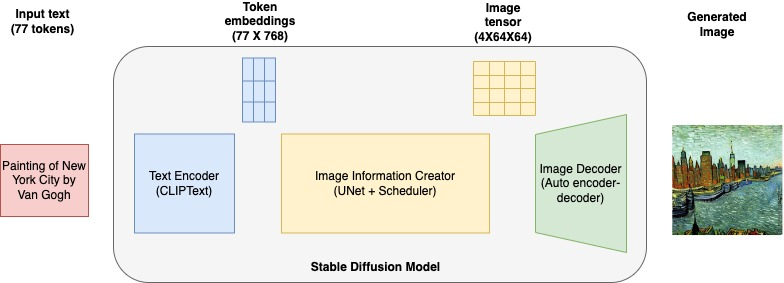
\includegraphics[width=\textwidth]{images/modelsdiffusion.jpg}
\captionof{figure}{Exemple de modèle de diffusion}
\vspace{1cm}

% --------- Deuxième modèle ---------
\subsection{Réseaux antagonistes génératifs}
\paragraph{}
Le réseau antagoniste génératif (GAN) est un autre modèle d'IA générative qui s'appuie
sur le concept du modèle de diffusion.

Les GAN fonctionnent en entraînant deux réseaux neuronaux de manière compétitive.
Le premier réseau, appelé \textit{générateur}, génère de faux échantillons de
données en ajoutant du bruit aléatoire. Le second réseau, appelé \textit{discriminateur},
essaie de faire la distinction entre les données réelles et les fausses données
produites par le générateur.

Pendant l'entraînement, le générateur améliore continuellement sa capacité à créer
des données réalistes, tandis que le discriminateur sait de mieux en mieux
distinguer le vrai du faux. Ce processus contradictoire se poursuit jusqu'à ce que
le générateur produise des données si convaincantes que le discriminateur ne peut
pas les différencier des données réelles.

Les GAN sont largement utilisés pour la génération d'images réalistes, le
transfert de style et les tâches d'augmentation des données.

\vspace{1cm}

\includegraphics[width=\textwidth]{images/gan-datascientest-1024x512.png}
\captionof{figure}{GAN (réseaux antagonistes génératifs)}
\vspace{1cm}

% --------- Troisième modèle ---------
\subsection{Autoencodeurs variationnels}
\paragraph{}
Les autoencodeurs variationnels (VAE) apprennent une représentation compacte des
données appelée \textit{espace latent}. L'espace latent est une représentation
mathématique des données. Vous pouvez le voir comme un code unique représentant les
données en fonction de tous leurs attributs. Par exemple, si vous étudiez des visages,
l'espace latent contient des nombres représentant la forme des yeux, du nez, des
pommettes et des oreilles.

Les VAE utilisent deux réseaux neuronaux : l’\textit{encodeur} et le \textit{décodeur}.
L'encodeur mappe les données d'entrée selon une moyenne et une variance pour
chaque dimension de l'espace latent. Il génère un échantillon aléatoire à partir
d'une distribution gaussienne (normale). Cet échantillon est un point dans l'espace
latent et représente une version compressée et simplifiée des données d'entrée.

Le décodeur extrait ce point échantillonné de l'espace latent et le reconstruit
en données qui ressemblent à l'entrée d'origine. Des fonctions mathématiques sont
utilisées pour mesurer à quel point les données reconstruites correspondent aux données
d'origine.

\vspace{1cm}
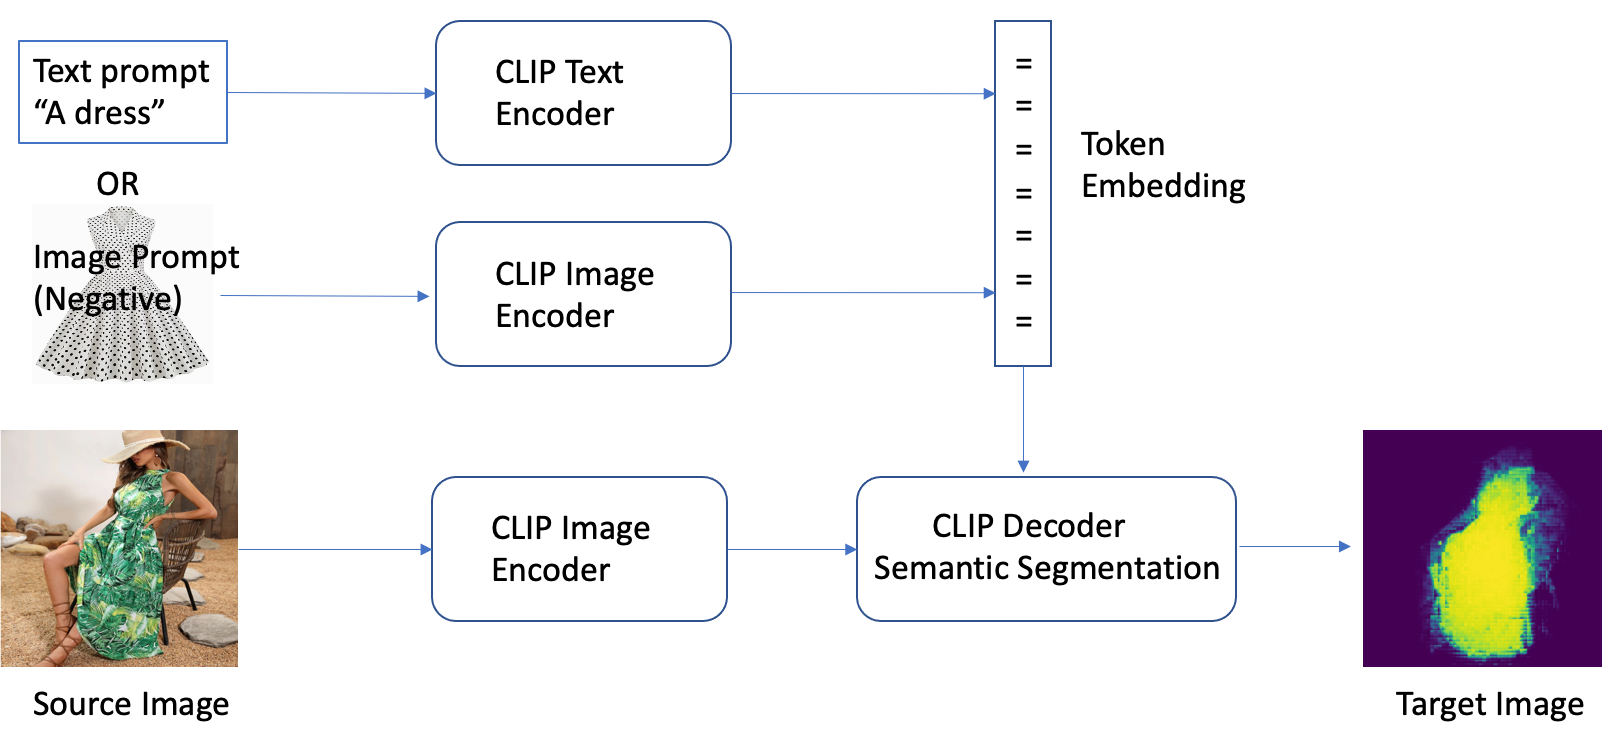
\includegraphics[width=\textwidth]{images/clipseg_architecture-1.png}
\captionof{figure}{Exemple d'autoencodeur variationnel (VAE)}
\vspace{1cm}

% --------- Quatrième modèle ---------
\subsection{Modèles basés sur des transformateurs}
\paragraph{}
Les modèles d'IA générative basés sur des transformateurs s'appuient sur les concepts
d'encodeur et de décodeur des VAE. Les modèles basés sur des transformateurs
ajoutent des couches supplémentaires à l'encodeur afin d'améliorer les
performances des tâches basées sur du texte telles que la compréhension, la traduction
et l'écriture créative.

\paragraph{}
Les modèles basés sur des transformateurs utilisent un mécanisme d'\textit{auto-attention}.
Ils évaluent l'importance des différentes parties d'une séquence d'entrée lors
du traitement de chaque élément de la séquence.

\paragraph{}
Une autre fonctionnalité clé est que ces modèles d’IA implémentent des \textit{intégrations
contextuelles}. Le codage d'un élément de séquence dépend non seulement de l'élément
lui-même, mais également de son contexte dans la séquence.

\paragraph{Fonctionnement des modèles basés sur des transformeurs}
Pour comprendre le fonctionnement des modèles basés sur des transformeurs,
imaginez une phrase sous la forme d’une séquence de mots.

L'\textit{auto-attention} aide le modèle à se concentrer sur les mots pertinents
lorsqu'il traite chaque mot. Pour capturer différents types de relations entre
les mots, les modèles génératifs basés sur des transformeurs utilisent plusieurs
couches d’encodeur appelées \textit{têtes d’attention}. Chaque tête apprend à se
concentrer sur différentes parties de la séquence d’entrée, ce qui permet au
modèle de prendre en compte simultanément divers aspects des données.

Chaque couche affine également les intégrations contextuelles, les rendant plus informatives
et capturant tout, de la syntaxe grammaticale aux significations sémantiques
complexes.
\vspace{1cm}
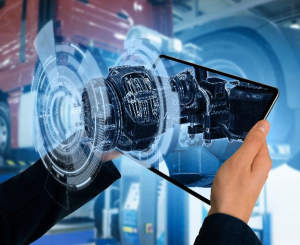
\includegraphics[width=1\textwidth, height=5cm]{images/3D-Model-1-300x245.png}
\captionof{figure}{Modèle basé sur un transformateur}
\vspace{0.5cm}

\section{Quelles sont les limites de l’IA générative ?}

Malgré leurs avancées, les systèmes d’IA générative peuvent parfois produire des
informations inexactes ou trompeuses. Ils s’appuient sur des modèles et des données
sur lesquels ils ont été formés et peuvent refléter des biais ou des inexactitudes
inhérents à ces données. Les autres préoccupations liées aux données
d’entraînement incluent :

\subsection*{Sécurité}

Des problèmes de confidentialité et de sécurité des données se posent si des
données propriétaires sont utilisées pour personnaliser des modèles d’IA
générative. Des efforts doivent être déployés pour garantir que les outils d’IA générative
génèrent des réponses qui limitent l’accès non autorisé à des données propriétaires.
Des problèmes de sécurité se posent également en cas de manque de responsabilité
et de transparence dans la manière dont les modèles d’IA prennent des décisions.

\subsection*{Créativité}

Bien que l’IA générative puisse produire du contenu créatif, elle manque souvent
de véritable originalité. La créativité de l’IA est limitée par les données sur lesquelles
elle a été entraînée, ce qui donne lieu à des résultats qui peuvent sembler
répétitifs ou dérivés. La créativité humaine, qui implique une compréhension
plus approfondie et une résonance émotionnelle, reste difficile à reproduire pleinement
pour l’IA.

\subsection*{Coût}

L’entraînement et l’exécution de modèles d’IA générative nécessitent des
ressources de calcul importantes. Les modèles d’IA générative basés sur le cloud
sont plus accessibles et plus abordables que la création de nouveaux modèles à partir
de zéro.

\subsection*{Explicabilité}

En raison de leur nature complexe et opaque, les modèles d’IA générative sont souvent
considérés comme des boîtes noires. Il est difficile de comprendre comment ces
modèles aboutissent à des résultats spécifiques. Il est essentiel d’améliorer l’interprétabilité
et la transparence pour renforcer la confiance et l’adoption.

\section{Quelles sont les bonnes pratiques en matière d'adoption de l'IA
générative ?}

Si votre entreprise souhaite implémenter des solutions d'IA générative, tenez compte
des bonnes pratiques suivantes pour appuyer les efforts mis en œuvre.

\subsection*{Commencez par les applications internes}

Il est préférable de commencer l'adoption de l'IA générative par le
développement d'applications internes, en mettant l'accent sur l'optimisation des
processus et la productivité des employés. Vous bénéficiez d'un environnement
plus contrôlé pour tester les résultats tout en développant les compétences et
la compréhension de la technologie. Vous pouvez tester les modèles de manière approfondie
et même les personnaliser sur des sources de connaissances internes. Ainsi, vos clients
bénéficieront d’une bien meilleure expérience lorsque vous utiliserez les modèles
pour des applications externes.

\subsection*{Améliorez la transparence}

Expliquez clairement comment fonctionnent toutes les applications et tous les
résultats de l’IA générative, afin que vos utilisateurs sachent qu’ils interagissent
avec l’IA et non avec des humains. Par exemple, l'IA peut se présenter comme étant
une IA, ou les résultats de recherche basés sur l'IA peuvent être marqués et mis
en évidence. Ainsi, vos utilisateurs peuvent prendre des décisions éclairées
lorsqu'ils interagissent avec le contenu. Ils peuvent également être plus proactifs
dans le traitement des inexactitudes ou des biais cachés que les modèles sous-jacents
peuvent présenter en raison des limites de leurs données d'apprentissage.

\subsection*{Implémentez la sécurité}

Mettez en place des barrières de protection permettant à vos applications d'IA
générative de refuser l'accès non autorisé aux données sensibles. Impliquez les équipes
de sécurité dès le départ afin que tous les aspects puissent être pris en compte
immédiatement. Par exemple, vous devrez peut-être masquer des données et supprimer
des données d'identification personnelle (PII) avant d'entraîner des modèles sur
des données internes.

\subsection*{Effectuez des tests exhaustifs}

Développez des processus de test automatisés et manuels pour valider les
résultats et testez tous les types de scénarios auxquels le système d’IA
générative peut être confronté. Formez plusieurs groupes de bêta-testeurs pour essayer
les applications de différentes manières et documenter les résultats. Le modèle
s'améliorera également en continu grâce aux tests, et vous aurez un meilleur contrôle
sur les résultats attendus et les réponses.

\section{Amélioration de la pertinence des chatbots d'IA générative}
\section*{Qu’est-ce qu’un modèle pré-entraîné ?}

Quand on parle de modèles d’IA, on parle généralement d’algorithmes utilisant des
réseaux de neurones. Cette technologie est utilisée par les \textit{Larges
Modèles de Langage} (LLM) comme \textit{ChatGPT} ou \textit{Mistral Large}, par
les algorithmes de génération d’images ou de reconnaissance visuelle. Ces modèles
sont entraînés sur des jeux de données très volumineux, leur permettant
d’acquérir une base solide dans le domaine de compétences qu’ils vont maîtriser.

Il est possible de régler de nombreux paramètres sur les différentes couches
d’un réseau pour modifier la manière dont est traitée l’information. On arrive à
plusieurs milliards de paramètres lorsque les modèles sont vraiment volumineux (de
quoi laisser de la place à la personnalisation\ldots) !

\subsection{RAG (Retrieval-Augmented Generation)}
\paragraph{}
Le \textit{Retrieval Augmented Generation} (RAG) est une approche novatrice qui combine
le meilleur de deux mondes en IA : la recherche d’informations (\textit{retrieval},
qui ne génère pas de réponse originale) et la génération de contenu (qui ne
s’appuie que sur les données de son entraînement).

Traditionnellement, les \textit{Large Language Models} (LLM) génèrent du contenu
en s’appuyant uniquement sur les informations apprises durant leur phase d’entraînement.
Le RAG, en revanche, permet au modèle de « consulter » une base de données ou un
corpus de documents externes en temps réel pour enrichir sa génération de texte.

Cette capacité de recherche améliore significativement la précision, la pertinence
et la richesse du contenu généré.

\section*{Comment fonctionne le RAG ?}

Le processus du \textit{Retrieval Augmented Generation} (RAG) peut être divisé en
deux grandes étapes :

\begin{itemize}
	\item \textbf{La récupération} : Lorsque le modèle reçoit une requête, il effectue
		une recherche dans un ensemble prédéfini de documents ou de données pour trouver
		les informations les plus pertinentes par rapport à la requête. Cette
		recherche est souvent facilitée par des techniques d’indexation et de
		récupération d’informations sophistiquées.

	\item \textbf{La génération} : Une fois les informations pertinentes
		récupérées, le modèle les utilise, en plus de sa propre connaissance interne,
		pour générer une réponse ou un contenu qui non seulement répond à la requête
		initiale mais le fait de manière plus informée et précise.
\end{itemize}
\section*{Avantages du RAG}

L’intégration du \textit{Retrieval Augmented Generation} dans les systèmes d’IA
générative offre plusieurs avantages significatifs, améliorant non seulement la qualité
du contenu généré mais aussi son applicabilité dans divers contextes.

\subsection*{Amélioration de la pertinence et de l'exactitude}
En puisant dans une base de données externe pour compléter ses connaissances, un
modèle RAG peut fournir des réponses plus précises et pertinentes aux questions
posées. Cela est particulièrement utile pour les requêtes nécessitant des données
actualisées ou spécifiques à un domaine.

\subsection*{Contenu plus riche et informé}
La génération de contenu ne se contente plus de refléter les connaissances préalablement
acquises pendant l’entraînement du modèle. Cela conduit à la création de textes
plus informatifs, détaillés et nuancés.

\subsection*{Flexibilité et adaptabilité}
Grâce à sa capacité à consulter une vaste gamme de sources, un modèle RAG peut
s’adapter à une variété de sujets et de domaines. Cette flexibilité le rend particulièrement
précieux pour les applications nécessitant une expertise dans des domaines de niche
ou en constante évolution.

\subsection*{Interactivité améliorée}
Le RAG permet aux systèmes d’interagir de manière plus sophistiquée avec les utilisateurs,
en répondant à des questions complexes ou en fournissant des explications
détaillées qui s’appuient sur des données et des sources externes.

\subsection*{Applications du RAG}

Les applications du RAG sont multiples et permettent d’améliorer grandement la qualité
du contenu généré. Voici quelques exemples illustrant comment cette approche
peut s’intégrer à différents environnements professionnels :

\begin{itemize}[leftmargin=1.5cm]
	\item \textbf{Support client} : Le RAG permet de fournir des réponses
		personnalisées et précises aux requêtes des clients en accédant en temps
		réel à une base de données exhaustive, améliorant ainsi l’expérience client.
		Les systèmes de support équipés de RAG peuvent générer des FAQ dynamiques, répondant
		aux questions courantes avec des informations à jour, réduisant le volume de
		requêtes nécessitant une intervention humaine.

	\item \textbf{Génération de contenu} : Dans le marketing, le RAG peut être utilisé
		pour créer des articles, des billets de blog, et des descriptions de produits
		personnalisés pour le public cible, en s’appuyant sur des données de
		recherche pertinentes.

	\item \textbf{Ventes} : Le RAG peut dynamiser les stratégies de vente en
		créant des propositions commerciales sur mesure qui résonnent avec les
		besoins et préférences spécifiques des prospects. Basé sur l’analyse des interactions
		précédentes avec un client, le modèle peut générer des scripts de vente
		optimisés et des points de discussion pertinents.

	\item \textbf{Ressources humaines} : Le RAG facilite la rédaction de
		descriptions de poste attractives et précises, en s’inspirant des meilleures
		pratiques et des exemples de succès dans l’industrie. Il permet également de
		créer des FAQ internes détaillées, répondant efficacement aux questions des employés
		en se référant à des politiques et procédures actualisées, favorisant ainsi
		un environnement de travail informé et harmonieux.
\end{itemize}

\subsection*{Défis et limites}

Malgré ses nombreux avantages, le RAG n’est pas sans défis. La qualité et la pertinence
des informations récupérées dépendent fortement de la qualité du corpus de documents
sous-jacent. De plus, l’intégration efficace des informations récupérées dans la
génération de texte reste un défi technique non négligeable. Enfin, des considérations
éthiques et de confidentialité entrent en jeu lorsqu’il s’agit de déterminer quelles
informations peuvent être récupérées et utilisées par ces modèles.

\subsection{Fine-Tuning ?}
Contrairement à l’entraînement initial qui nécessite des jeux de données massifs
comme ImageNet, cet affinage se concentre sur des données plus restreintes et
spécialisées.

Il s’agit d’un processus itératif qui vise à améliorer la performance du modèle
sur une tâche particulière, sans perdre les connaissances préalables acquises lors
de l’entraînement initial.

L’idée centrale réside dans la capacité du modèle à généraliser à de nouveaux domaines
tout en conservant sa capacité à se spécialiser.

Cette approche trouve des applications variées à travers de nombreux domaines comme
:
\begin{itemize}
	\item \textbf{Computer Vision} : un modèle peut être fine-tuné pour la
		détection d’objets spécifiques dans des contextes particuliers (véhicules autonomes,
		caméras de surveillance).

	\item \textbf{Médical} : un modèle peut être affiné pour la détection
		d’organes spécifiques dans les images médicales.

	\item \textbf{NLP} : un modèle peut être adapté pour la classification de
		documents juridiques, la détection de tonalité émotionnelle, ou la
		traduction automatique spécialisée.
\end{itemize}

\subsection*{Les étapes du processus de Fine-Tuning}
Le Fine-Tuning suit une approche méthodique :
\begin{enumerate}
	\item \textbf{Collecte et préparation des données} : données spécifiques, de haute
		qualité, nettoyées.

	\item \textbf{Choix du modèle pré-entraîné} selon la tâche cible.

	\item \textbf{Évaluation initiale} du modèle sur la tâche cible pour disposer
		d'une base de référence.

	\item \textbf{Ajustement des hyperparamètres} (taux d’apprentissage, nombre
		d’itérations, taille du lot).
\end{enumerate}

Pour optimiser ces hyperparamètres, on peut utiliser :
\begin{itemize}
	\item la recherche aléatoire,

	\item la recherche en grille,

	\item l’optimisation bayésienne.
\end{itemize}

\subsection*{Les stratégies avancées d’affinage}
Au-delà du simple ajustement, plusieurs stratégies avancées existent :
\begin{itemize}
	\item \textbf{Transfert d’apprentissage} : utiliser la connaissance acquise
		sur une tâche pour une autre tâche similaire.

	\item \textbf{Fine-Tuning progressif} : affiner progressivement, en commençant
		par les couches supérieures, puis inférieures.

	\item \textbf{Techniques de régularisation} comme le dropout pour limiter le
		surajustement.
\end{itemize}

Une évaluation à chaque étape permet de détecter signes de surajustement ou de sous-ajustement.

\subsection*{Les meilleurs outils et bibliothèques de Fine-Tuning}
Parmi les outils les plus utilisés :
\begin{itemize}
	\item \textbf{TensorFlow} : fonctionnalités avancées de transfert
		d’apprentissage.

	\item \textbf{Keras} : interface haut niveau simplifiant le Fine-Tuning.

	\item \textbf{PyTorch} : flexibilité et manipulation aisée des couches du
		modèle.

	\item \textbf{Hugging Face Transformers} : bibliothèque de modèles pré-entraînés.
\end{itemize}

Pour la visualisation :
\begin{itemize}
	\item \textbf{TensorBoard} pour TensorFlow,

	\item \textbf{TensorBoardX} pour PyTorch.
\end{itemize}

Les communautés GitHub et Stack Overflow offrent aussi de nombreux exemples,
tutoriels et solutions aux problèmes courants.

\subsection*{Les défis du Fine-Tuning : difficultés à surmonter}
Parmi les défis principaux :
\begin{itemize}
	\item \textbf{Surajustement} : atténué par des techniques comme le dropout ou
		la normalisation par lots.

	\item \textbf{Déséquilibre des classes} : l’usage de poids de classe peut
		corriger ce biais.

	\item \textbf{Amplification des biais} : diversifier les sources de données et
		utiliser des techniques de correction de biais.
\end{itemize}
\subsection{Le prompt engineering }

Le prompt engineering, aussi appelé « ingénierie de requête », est une technique
qui consiste à fournir des instructions détaillées aux modèles de traitement du langage
naturel (Natural Language Processing, ou NLP) afin d’améliorer leurs
performances.

Concrètement, le prompt engineering permet de guider plus précisément un modèle NLP
en lui donnant des indications sur la tâche à effectuer et le contexte dans lequel
elle s’inscrit. Plutôt que de laisser le modèle répondre de manière générique à
une question posée, le prompt engineering permet de cadrer la réponse attendue.

Par exemple, il est possible d’utiliser le prompt engineering pour entraîner un
modèle de génération de texte à rédiger des e-mails de relance client plus
efficaces et personnalisés. Au lieu de lui donner comme simple instruction « Rédigez
un e-mail de relance client », le prompt engineering doit fournir des détails :
« Rédigez un e-mail de 200 mots pour relancer le client Jean Dupont qui n’a pas
payé sa dernière facture depuis 30 jours. Utilisez un ton courtois et proposez une
remise de 10\% s’il paie dans les 7 prochains jours. »

Ainsi, le prompt engineering permet de mieux contrôler et orienter les réponses d’un
modèle NLP en fournissant un contexte, des exemples et des instructions claires.

\subsection*{Comment fonctionne le prompt engineering ?}

L’utilisation du prompt engineering repose sur deux mécanismes complémentaires.
D’une part, l’entraînement via des exemples commentés : cette technique consiste
à fournir au modèle NLP des exemples concrets de prompts efficaces, accompagnés
d’explications sur les raisons qui les rendent performants. Par exemple, les
prompts donnés au modèle peuvent être conçus pour générer des slogans
publicitaires impactants, en expliquant pourquoi ils cadrent bien la tâche attendue.

D’autre part, l’orientation pas à pas : le modèle est guidé étape par étape sur
la façon de construire un prompt optimal. Il est, par exemple, possible de lui indiquer
qu’un bon prompt doit définir clairement l’objectif, donner des exemples
pertinents, établir le contexte, utiliser un vocabulaire simple, etc.

En combinant ces deux techniques, le modèle « apprend » à générer de meilleurs
prompts de manière autonome. À force d’exemples commentés et d’orientation, le
modèle finit par intégrer les bonnes pratiques du prompt engineering et les
appliquer de lui-même.

L’enjeu est de fournir suffisamment d’informations dans le prompt pour que le
modèle produise une réponse de qualité, mais sans non plus le surcharger d’instructions
qui limitent sa créativité. Le prompt engineering cherche ainsi le bon équilibre
entre guidage et autonomie.

\subsection*{Quels sont les différents types de prompt engineering ?}

Il existe plusieurs façons d’aborder le prompt engineering en fonction du résultat
recherché. Voici les trois grands types de prompt engineering :

\begin{itemize}
	\item Le prompt engineering pour l’entraînement des modèles : il consiste à fournir
		au modèle NLP des prompts spécifiquement conçus pour l’entraîner sur une tâche
		donnée. Par exemple, lui donner des milliers de prompts illustrant la génération
		de textes publicitaires.

	\item Le prompt engineering pour l’inférence en production : une fois le modèle
		déployé, il est alimenté avec des prompts optimisés pour les cas d’usage
		visés. Cette méthode est utilisée pour les prompts de modération de contenu,
		de réponse aux questions clients, etc.

	\item Le prompt engineering adaptatif : le modèle NLP est entraîné à générer lui-même
		les meilleurs prompts en fonction du contexte. Cette approche a pour but de
		rendre le modèle capable d’un prompt engineering autonome.
\end{itemize}

Chacune de ces variantes présente des spécificités en termes de méthodologie. Le
prompt engineering pour l’entraînement met l’accent sur la diversité et la quantité
de données. Celui pour l’inférence se concentre sur la qualité des prompts en
contexte réel. L’approche adaptative cherche à donner au modèle la capacité d’apprendre
à faire un prompt engineering efficace par lui-même.

Les chercheurs combinent souvent ces différents types de prompt engineering de manière
complémentaire pour obtenir les meilleures performances. Cette diversité des
techniques de prompt engineering est une force pour cette discipline encore
émergente.

\subsection*{Quelles compétences requiert la maîtrise du prompt engineering ?}

Réussir dans le prompt engineering, sans pour autant être un prompt engineer (ingénieur
de requête), requiert de solides compétences pluridisciplinaires.

Tout d’abord, une connaissance approfondie des modèles de traitement du langage
naturel est indispensable pour créer des prompts adaptés à leurs forces et à
leurs limites.

La rédaction est également cruciale, car le prompt se doit d’être un texte concis,
précis et cohérent. De bonnes capacités rédactionnelles sont donc essentielles.

La maîtrise de techniques d’apprentissage automatique comme le transfer learning
est aussi un atout, celles-ci étant souvent employées conjointement au prompt
engineering.

De même, une expertise en linguistique computationnelle permet de mieux appréhender
les mécanismes d’interprétation du langage par les modèles.

Côté technique, la programmation et la data science sont nécessaires pour
intégrer et évaluer les performances des prompts. La rigueur dans les tests et les
expérimentations permet d’identifier les prompts les plus efficaces.

Enfin, la créativité et un esprit critique sont des qualités essentielles pour
le prompt engineering.

\subsection*{Quels sont les avantages du prompt engineering ?}

L’utilisation du prompt engineering présente plusieurs avantages. Tout d’abord, cette
technique permet d’obtenir des réponses plus précises et pertinentes de la part des
modèles NLP. Avec un prompt bien conçu, le modèle va générer une réponse correspondant
exactement à la tâche demandée, et non pas quelque chose de vague ou
d’approximatif.

Le prompt engineering assure également une meilleure adéquation entre la réponse
du modèle et les besoins spécifiques de l’utilisateur, en cadrant la génération de
texte en fonction du cas d’usage visé et des instructions fournies. Par ailleurs,
un prompt détaillé va limiter les contresens et mauvaises interprétations du modèle
NLP, réduisant ainsi les biais et les erreurs. Le prompt engineering favorise aussi
une plus grande cohérence des réponses du modèle, même face à des inputs
différents.

À terme, cette technique améliore les performances globales des modèles NLP en renforçant
leur capacité à comprendre des demandes complexes. Enfin, le prompt engineering offre
une meilleure contrôlabilité de ces modèles, en permettant à leurs concepteurs
d’orienter finement leur comportement via les consignes fournies.

\subsection*{Quelles sont les limites du prompt engineering ?}

Bien que présentant des avantages certains, l’utilisation du prompt engineering
comporte également des limites qu’il faut garder à l’esprit. Tout d’abord, il
s’agit d’une technique qui nécessite un investissement temps important ainsi que
de solides compétences en conception de prompts pour élaborer des instructions
optimales. Sans une expertise approfondie, il est assez facile de rédiger de
mauvais prompts qui vont en réalité dégrader les performances du modèle NLP au
lieu de les améliorer.

De plus, le prompt engineering est fortement dépendant du cas d’usage : des prompts
spécifiques à une tâche devront être entièrement réécrits en cas de changement d’objectif
ou de contexte. Par ailleurs, des prompts trop directifs ou détaillés peuvent réduire
la créativité et l’autonomie des modèles NLP en les enfermant dans des schémas de
réponse prédéfinis et stéréotypés. L’équilibre subtil entre guidage et liberté
accordée au modèle est difficile à trouver.

Le processus de conception de prompts efficaces s’appuie également sur de
nombreux essais-erreurs, des ajustements progressifs et de fins réglages : un prompt
optimal ne peut être obtenu immédiatement.

Enfin, la complexité des prompts tend à croître à mesure qu’on cherche à les
optimiser, jusqu’à potentiellement devenir contre-productifs s’ils sont surchargés
d’instructions. Malgré son potentiel prometteur, le prompt engineering ne constitue
donc pas une solution magique aux limitations des modèles NLP actuels.

\subsection*{Comment le prompt engineering va-t-il évoluer ?}

Même s’il s’agit d’une technologie déjà mature, le prompt engineering devrait encore
progresser à l’avenir, notamment grâce aux avancées dans les domaines connexes
du transfer learning et du few-shot learning.

Plusieurs évolutions sont à anticiper :

\begin{itemize}
	\item L’émergence de nouvelles méthodes pour générer des prompts plus efficaces,
		via l’utilisation d’algorithmes d’optimisation par exemple ;

	\item Le développement de bibliothèques de prompts pré-écrits, réutilisables
		d’un modèle NLP à l’autre ;

	\item La possibilité pour les modèles d’auto-générer les prompts les plus adaptés
		en fonction de la tâche demandée ;

	\item L’utilisation du prompt engineering pour entraîner des modèles NLP toujours
		plus puissants, atteignant des niveaux de compétence linguistique proches de
		l’humain ;

	\item L’écriture de prompts par les utilisateurs finaux eux-mêmes, permettant
		de guider les modèles NLP en langage naturel ;

	\item Une intégration accrue entre prompt engineering et techniques de search.
\end{itemize}

Grâce à ces avancées, le prompt engineering a le potentiel de devenir une technique
incontournable pour exploiter au maximum les capacités des modèles de traitement
du langage naturel sur une grande diversité de cas d’usage.

\subsection{Few Shot Learning ?}
Le Few Shot Learning (FSL) est un framework du domaine du Machine Learning,
c’est-à-dire une structure de base pour le développement de codes de
programmation. Il est utilisé pour entraîner les modèles d’IA à faire des prédictions
précises à partir d’une petite quantité de données d’entraînement. Alors que les
méthodes de Machine Learning traditionnelles nécessitent souvent des milliers de
points de données pour fournir des résultats fiables, le Few Shot Learning vise à
optimiser l’apprentissage avec un minimum de données.

L’objectif principal du Few Shot Learning est un apprentissage efficace à partir
de quelques exemples seulement. En travaillant avec une quantité minimale de
données, le FSL s’avère particulièrement utile dans les situations où il est difficile
de collecter de grandes quantités de données étiquetées (ex : maladies rares, manuscrits
uniques).

Le Few Shot Learning peut être considéré comme un sous-groupe du n-Shot-Learning
(N-Way-K-Shot), où : - $N$ est le nombre de classes, - $K$ est le nombre
d’exemples par classe.

Cela comprend également : - le One Shot Learning (un exemple par classe), - le Zero
Shot Learning (aucun exemple étiqueté).

\subsection*{Comment fonctionne le Few Shot Learning ?}
Même si des algorithmes spéciaux et des réseaux neuronaux réussissent de nombreuses
tâches de FSL, il est avant tout défini par le **problème d’apprentissage**
spécifique, et non par un modèle particulier.

Les principales approches sont :

\subsubsection*{Apprentissage par transfert}
Il s'agit d'adapter des modèles pré-entraînés pour de nouvelles tâches, en utilisant
les connaissances déjà acquises pour éviter le surajustement, surtout avec peu d'exemples.
Cela fonctionne particulièrement bien si la tâche cible est similaire à la tâche
d’origine.

\subsubsection*{Approche par les données}
Il s'agit de **générer des données supplémentaires** pour pallier le manque d'exemples,
souvent grâce à des réseaux génératifs (GANs). Cela est crucial dans des cas rares
(ex : espèces nouvellement découvertes).

\subsubsection*{Meta Learning (Méta-apprentissage)}
Le modèle apprend à apprendre : il généralise des schémas à travers différentes tâches.

On distingue deux types :

\paragraph*{Méta-apprentissage basé sur les métriques}
Plutôt que de modéliser des classes directement, on apprend des distances entre
exemples : - Réseaux siamois - Réseaux de matching - Réseaux prototypiques -
Réseaux de relation (Relation Networks)

\paragraph*{Méta-apprentissage basé sur l’optimisation}
On optimise les modèles pour qu'ils s'adaptent rapidement à de nouvelles tâches
: - MAML (Model Agnostic Meta-Learning) - Optimisation par LSTM - LEO (Latent Embedding
Optimization)

\subsection*{Principaux domaines d’application du Few Shot Learning}
Les secteurs concernés sont nombreux :

\begin{itemize}
	\item \textbf{Computer Vision} : classification d’images, reconnaissance d’objets.

	\item \textbf{Robotique} : adaptation rapide à de nouveaux environnements.

	\item \textbf{Traitement du langage} : adaptation de grands modèles de langage.

	\item \textbf{Santé publique} : diagnostic de maladies rares.

	\item \textbf{Secteur bancaire} : détection de fraudes avec peu d’exemples.
\end{itemize}

\subsection*{Enjeux concrets liés à la mise en œuvre du Few Shot Learning}
Le Few Shot Learning présente plusieurs défis :
\begin{itemize}
	\item \textbf{Surajustement} : le risque est élevé avec peu de données.

	\item \textbf{Qualité des données} : si les données sont de mauvaise qualité, la
		performance chute.

	\item \textbf{Sélection de caractéristiques} : difficile avec peu d’exemples.

	\item \textbf{Ressources de calcul} : optimisation fine requiert du temps et
		des ressources.
\end{itemize}

\subsection{Low Rank Adaptation}
Cette approche novatrice se concentre sur la réduction de la dimensionnalité des
données, dans le but de faciliter l’adaptation de domaine : le transfert d’un modèle
depuis un domaine source où il est entraîné vers un domaine cible où les données
peuvent être différentes.

Un concept central de cette méthode est la décomposition à faible rang des matrices.
Celle-ci permet de représenter les données sous une forme plus compacte, tout en
préservant leur structure sous-jacente.

Dans le contexte de l’apprentissage automatique, cette décomposition vise à
extraire les caractéristiques les plus importantes des données d’entraînement. Le
but est de construire un modèle plus généralisable pour le domaine cible.

Il existe différentes méthodes pour y parvenir. Les plus utilisées sont la
décomposition en valeurs singulières (Singular Value Decomposition ou SVD) et la
décomposition en facteurs non négatifs (Non-Negative Matrix Factorization ou NMF).

Grâce à la réduction de dimensionnalité des données, on évite les problèmes de surajustement
(overfitting) pouvant survenir quand les modèles sont directement appliqués à des
données de cibles différentes. C’est ce qui simplifie le transfert de
connaissances.

L’un des principaux points forts de la Low Rank Adaptation est sa capacité à
capturer les corrélations et dépendances entre les caractéristiques des données.
Ainsi, l’information cruciale pour l’adaptation est mieux représentée.

Un autre avantage est la possibilité d’appliquer cette approche à différentes
tâches de Machine Learning comme la classification, la régression ou même la génération
de données synthétiques.

\subsection*{À quoi ça sert ? Quelles sont les applications ?}
La Low Rank Adaptation est une méthode qui a fait ses preuves, et qui est déjà
adoptée dans de nombreux domaines du Machine Learning.

Dans la vision par ordinateur (Computer Vision), elle est utilisée pour la reconnaissance
d’objets au sein d’environnements différents de ceux utilisés pour l’entraînement
initial.

En utilisant des décompositions à faible rang sur les représentations des caractéristiques
des images, les modèles ML peuvent mieux généraliser à de nouvelles conditions
d’éclairage, d’angle de vue ou d’environnement pour améliorer considérablement leurs
performances dans le monde réel.

Pour le NLP ou traitement naturel du langage, cette approche s’avère aussi très
efficace pour les tâches de traduction automatique.

Alors que les données des domaines sources et cibles peuvent considérablement
varier, l’adaptation à faible rang permet de créer des modèles plus flexibles en
extrayant les aspects linguistiques essentiels et en les appliquant au nouveau domaine.
La traduction dans des contextes différents s’en trouve améliorée.

De même, pour la reconnaissance de la parole, la Low Rank Adaptation est utile
pour adapter les modèles de reconnaissance vocale à des locuteurs spécifiques ou
à différents environnements acoustiques.

Les techniques de décomposition à faible rang permettent aux systèmes de mieux
capturer les variations entre les interlocuteurs et donc d’obtenir une meilleure
précision dans des situations variées.

Enfin, en intégrant cette méthode d’adaptation aux architectures de réseaux de neurones,
l’apprentissage par transfert est facilité. Les connaissances acquises dans un domaine
sont transmises à un domaine cible, augmentant fortement les performances pour
une large variété de tâches.

\subsection*{Les défis de la Low Rank Adaptation}
Tous les exemples évoqués dans le chapitre précédent démontrent l’efficacité de
la Low Rank Adaptation pour surmonter les défis liés à l’adaptation de domaine
dans le Machine Learning.

Malgré ses nombreux avantages, cette approche présente aussi des défis spécifiques
à relever. Par exemple, la gestion du surajustement (overfitting) et du sous-ajustement
(underfitting) des modèles peut être difficile.

Une décomposition à faible rang trop restrictive peut entraîner une perte d’informations
cruciales, tandis qu’une décomposition trop complexe peut conduire à la
suradaptation aux données d’entraînement. Trouver le bon équilibre est donc essentiel
pour l’optimisation des performances sur de nouvelles données.

Autre problème potentiel : les domaines sources et cibles peuvent être extrêmement
différents, ce qui entraîne une hétérogénéité des données compliquant fortement
l’adaptation.

La diversité des caractéristiques entre les deux domaines peut en effet affecter
la capacité du modèle à transférer des connaissances de manière appropriée.

Pour éviter ce désagrément, il convient de développer des techniques de décomposition
à faible rang capables de capturer les variations tout en conservant les structures
essentielles.

Enfin, dans de nombreuses situations, il n’est pas toujours évident d’obtenir des
données étiquetées dans le domaine cible. Elles peuvent être limitées, ou tout simplement
trop coûteuses.

Or, la Low Rank Adaptation requiert généralement une large quantité de données
pour construire des modèles généralisables. Ceci exige des recherches supplémentaires
pour développer des méthodes exploitant les données non étiquetées ou semi-étiquetées,
comme l’adaptation à faible rang transductive.
\newpage
{}
\subsection{Comparaison des Techniques}
\begin{table}[h!]
	\centering
	\begin{tabular}{|p{3cm}|p{5cm}|p{5cm}|}
		\hline
		\textbf{Technique}                   & \textbf{Avantages}                                                                                  & \textbf{Limitations}                                                                              \\
		\hline
		RAG (Retrieval-Augmented Generation) & - Accès à des informations actualisées \newline - Améliore la pertinence des réponses               & - Dépendance aux bases de données \newline - Complexité de mise en œuvre                          \\
		\hline
		Fine-Tuning                          & - Modèle spécialisé pour une tâche précise \newline - Meilleure performance sur des cas spécifiques & - Coûteux en calculs \newline - Nécessite beaucoup de données                                     \\
		\hline
		Prompt Engineering                   & - Pas besoin de réentraîner le modèle \newline - Rapide à mettre en place                           & - Résultats instables \newline - Fortement dépendant de la qualité du prompt                      \\
		\hline
		Few-Shot Learning                    & - Apprentissage avec peu d'exemples \newline - Réduit le besoin de grandes bases de données         & - Moins performant qu'un entraînement complet \newline - Peut être sensible au choix des exemples \\
		\hline
		LoRA (Low-Rank Adaptation)           & - Fine-tuning léger \newline - Moins de ressources nécessaires                                      & - Peut être moins performant que le fine-tuning complet                                           \\
		\hline
		Distillation                         & - Modèle plus léger et rapide \newline - Adapté aux environnements contraints (mobile, embarqué)    & - Perte de performance par rapport au modèle original                                             \\
		\hline
	\end{tabular}
	\caption{Comparaison des principales techniques d'optimisation de modèles d'IA}
	\label{tab:comparaison-techniques}
\end{table}
\newpage
{}
\section*{Conclusion}
\addcontentsline{toc}{section}{Conclusion}
Dans ce chapitre, nous avons découvert l'univers fascinant de l'intelligence
artificielle générative. Cette technologie, qui permet de créer du contenu
original (textes, images, sons...), repose sur des modèles puissants comme les
autoencodeurs variationnels (VAE), les réseaux antagonistes génératifs (GAN) ou encore
les transformateurs.
\paragraph{}
Nous avons vu que l'IA générative offre énormément d'opportunités, mais qu’elle
comporte aussi des risques et des limites. Elle peut révolutionner des domaines comme
l'art, la santé ou l'éducation, tout en soulevant des questions importantes autour
de l'éthique, de la fiabilité et de l'utilisation abusive.
\paragraph{}
Grâce aux nouvelles techniques comme le fine-tuning, le prompt engineering ou le
few-shot learning, il est possible d'améliorer encore la pertinence et la
qualité des résultats produits. Mais pour en tirer le meilleur parti, il est
essentiel de l'utiliser avec précaution et de garder à l'esprit l'importance de
l'humain dans le processus.
\paragraph{}
L'IA générative n'en est qu'à ses débuts. Elle continuera d'évoluer et de transformer
notre quotidien. À nous de savoir l’accompagner de manière responsable, en restant
attentifs aux défis qu’elle pose et en utilisant son potentiel pour construire des
outils plus créatifs, plus justes et plus utiles.

\end{document}
